\chapter{工具类软件推荐}
\label{tools-software}

\begin{intro}
  本章我们介绍一些好用的「工具类软件」,例如视频播放器、下载工具、PDF 查看器等。我们尽量保证推荐的工具软件体积小巧,界面简洁,功能强大,同时尽量以开源、免费软件代替收费、破解软件。看完这一部分,你将能找到这些问题的答案:

  \begin{itemize}
    \item 有无好用的本地视频播放器软件(替代 QQ 影音 / 暴风影音 / ……)?
    \item 有无好用的下载工具(替代迅雷 / IDM / ……)?
    \item 有无好用的 PDF 查看器(替代福昕阅读器 / Acrobat / ……)?
    \item 有无好用的文件搜索工具(替代 Windows 自带「搜索功能」)?
    \item 有无好用的硬盘空间分析器(替代各大安全软件中的类似功能)?
    \item 有无好用的……(替代……)?
  \end{itemize}
\end{intro}

\begin{note}
  本章会持续更新。
\end{note}

与 Office 那样的工作软件和 QQ 那样的生活软件不同,工具类软件强调「实用」——在更好地实现本职功能的同时,追求小巧和简洁。本章将推荐一批我们认为比较「优质」的工具类软件,大家可以按需安装使用。

\section{文档类}

这一节介绍「文档类」实用工具,例如文本编辑器和 PDF 阅读器。

\subsection{Notepad3}

官网下载地址:\url{https://www.rizonesoft.com/downloads/notepad3/}

Notepad3 是一款用来替代系统内置「记事本」的文本编辑器。它具有语法高亮、代码折叠、括号匹配、自动缩进、自动编码、多次撤销以及高级搜索等许多功能,适用于替代记事本进行简单的文本编辑,以及进行轻度的代码编写。

\begin{figure}[htb!]
  \centering
  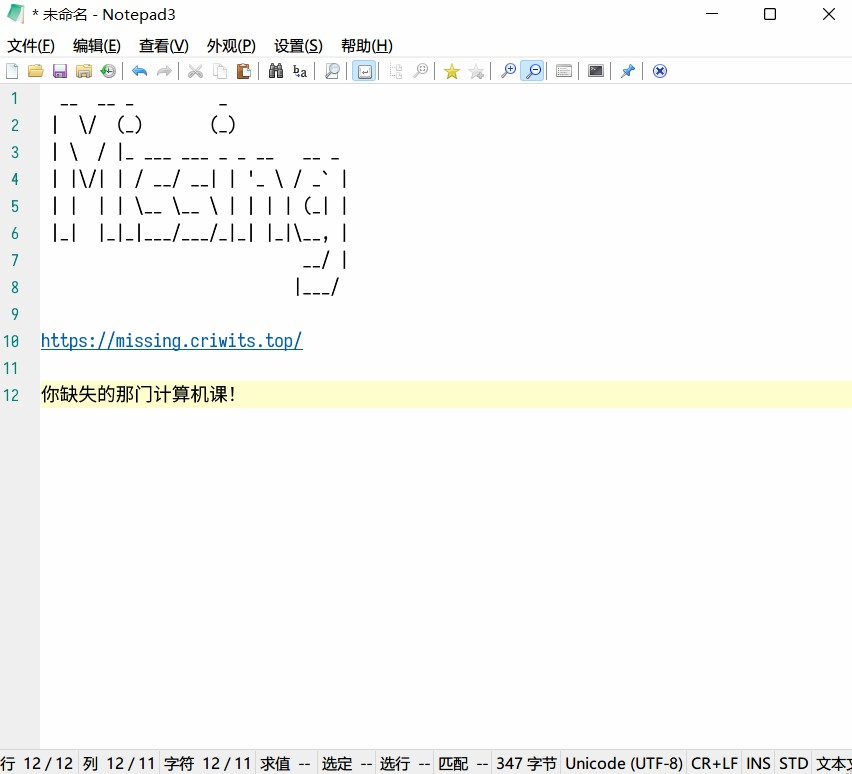
\includegraphics[width=10cm]{assets/Notepad3.jpg}
  \caption{Notepad 3界面}
  \label{Notepad3}
\end{figure}

与 Notepad3 类似的软件还有 Notepad++ 和 Sublime 等。这里我们\regcolor{不推荐}大家使用 Notepad++——尽管网上许多教程推荐它,尽管那也是一款非常优秀的文本编辑器。Notepad++ 的主要开发者屡次让政治立场混入技术世界,以「自由」之名行「渗透」之实,因而还需要大家审慎对待。

\subsection{SumatraPDF}

官网下载地址:\url{https://www.sumatrapdfreader.org/download-free-pdf-viewer}

SumatraPDF 是一个小巧(安装包不到 10 MB)却功能强大的 PDF 阅读器。除了基本的 PDF 阅读功能外,它还可以帮助我们「记忆」打开过的文档和它们的阅读位置,因而省去每次打开文件都重新翻页的烦恼。

\begin{figure}[htb!]
  \centering
  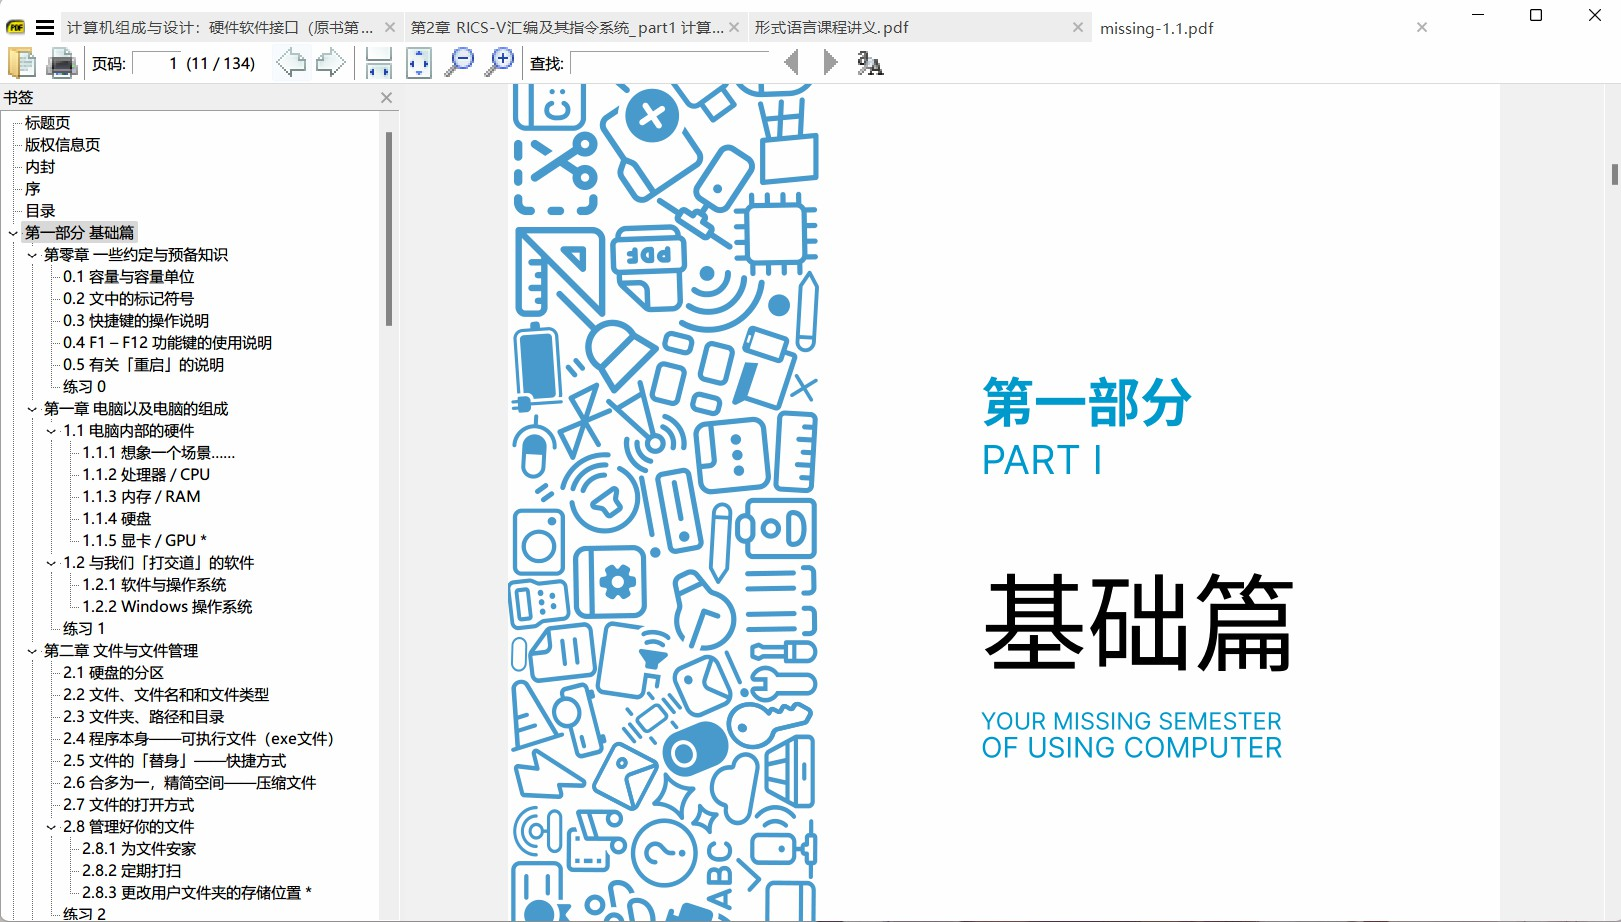
\includegraphics[width=13cm]{assets/SumatraPDF.jpg}
  \caption{SumatraPDF界面}
  \label{SumatraPDF}
\end{figure}

\section{影音类}

这一节介绍「影音类」实用工具,例如本地视频播放器。

\subsection{VLC Media Player}

官网下载地址:\url{https://www.videolan.org/vlc/}

VLC Media Player 是一个出色的本地视频播放器,它支持几乎所有常见格式的视频文件的播放,可以说是一个「万能」的播放器。与 VLC 类似的软件还有 PotPlayer,但 VLC 是开源而自由的软件,因而我们在这里推荐 VLC。

\begin{figure}[htb!]
  \centering
  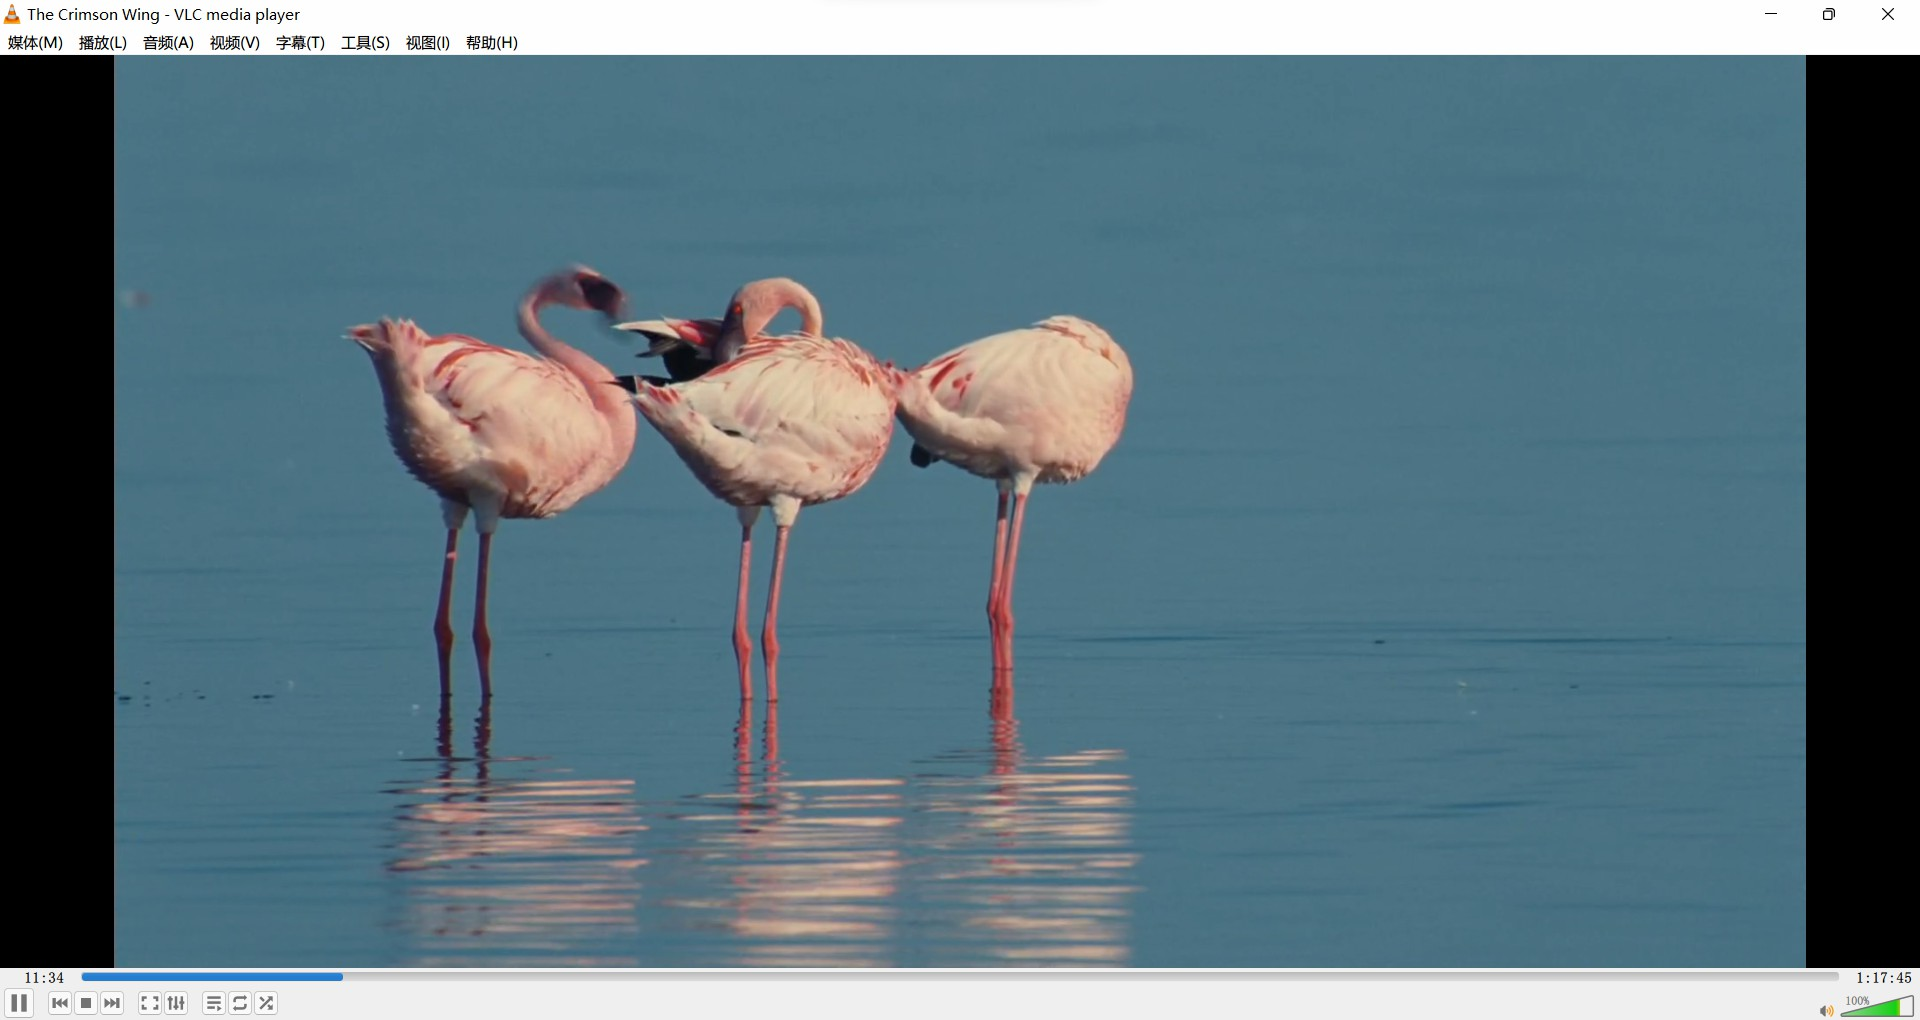
\includegraphics[width=13cm]{assets/VLC.jpg}
  \caption[VLC界面]{VLC界面\footnotemark}
  \label{VLC}
\end{figure}

\footnotetext{\textit{The Crimson Wing: Mystery of the Flamingos} © Disney / Disneynature. All rights reserved.}

\section{网络类}

这一节介绍「网络类」实用工具,例如下载器。

\subsection{Motrix}

官网下载地址:\url{https://motrix.app/zh-CN/}

Motrix,如它在网页上宣传的那样,是「一款全能的下载工具」,它基本上支持所有常见的资源协议的下载,包括 HTTP、FTP,以及群众喜闻乐见的磁力链接等。它界面精巧、代码开源、使用方便,是一款不可多得的优良下载工具。

\begin{figure}[htb!]
  \centering
  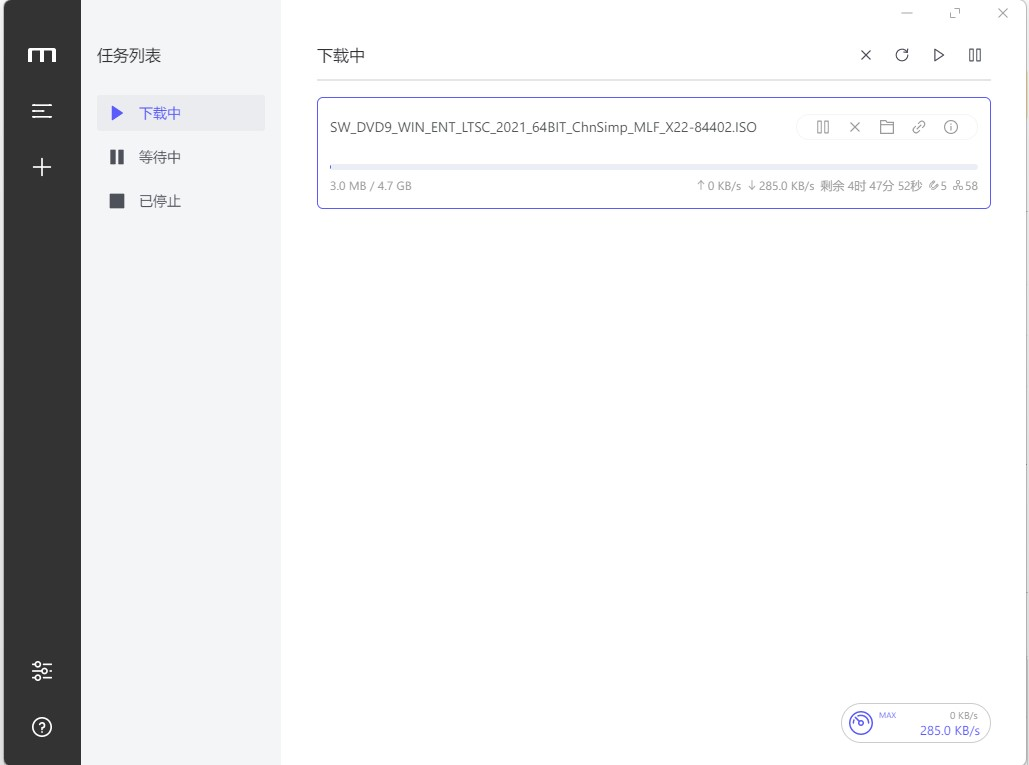
\includegraphics[width=10cm]{assets/Motrix.jpg}
  \caption{Motrix界面}
  \label{Motrix}
\end{figure}

\section{文件类}

这一节介绍「文件类」实用工具,例如文件搜索工具。

\subsection{SpaceSniffer}

官网下载地址:\url{http://www.uderzo.it/main_products/space_sniffer/download.html}

SpaceSniffer——直白的名字,专注于磁盘空间分析嗅探。在你不知道是什么让你的硬盘空间步步吃紧时,它能够快速分析磁盘中每个文件、文件夹的大小,并以相应比例的方格显示出来,让你知道谁是罪魁祸首。

\begin{figure}[htb!]
  \centering
  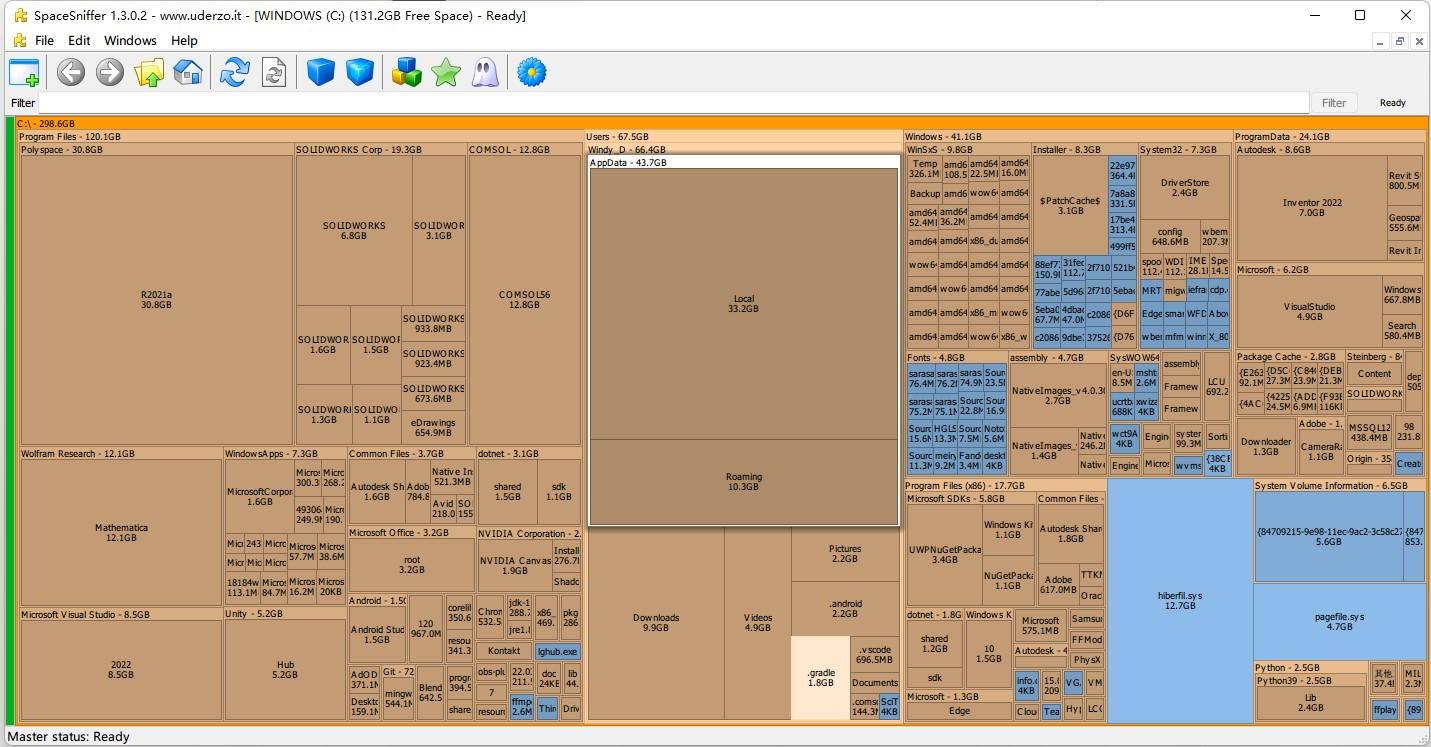
\includegraphics[width=13cm]{assets/SpaceSniffer.jpg}
  \caption{SpaceSniffer界面}
  \label{SpaceSniffer}
\end{figure}

\subsection{Everything}

官网下载地址:\url{https://www.voidtools.com/zh-cn/downloads/}

Everything,软件如其名,帮你寻找电脑上的一切!对于不经常整理文件的人来说,或许这个软件能为他们带来福音。它首先花点时间将你所有硬盘中的所有文件建立索引,之后便能在\regcolor{几乎瞬间}找到你所想要的文件 / 文件夹(当然前提是你还依稀记得它们的名字啥的)。

\begin{figure}[htb!]
  \centering
  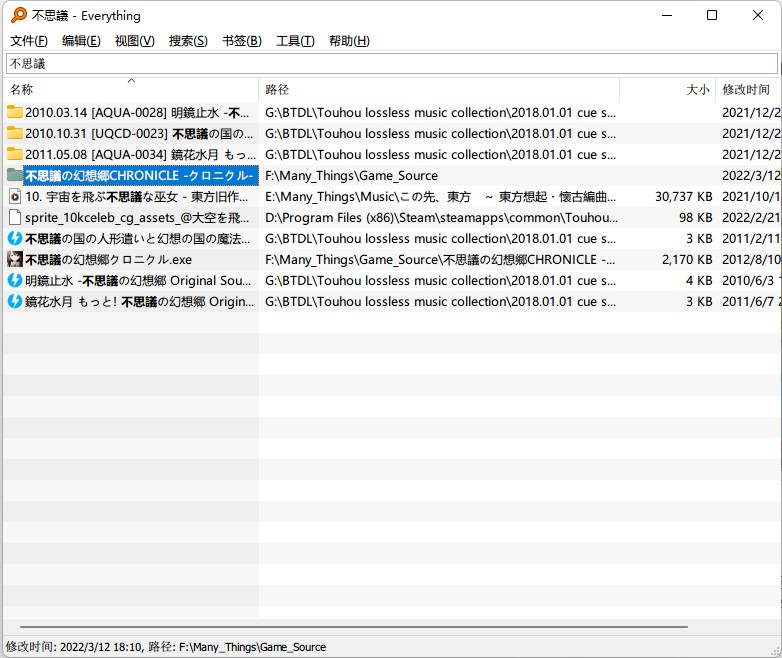
\includegraphics[width=10cm]{assets/Everything.jpg}
  \caption{Everything界面}
  \label{Everything}
\end{figure}

\practice

不妨试试上面介绍的这些小软件?